\section{Durchführung}
\label{sec:Durchführung}
Die Durchführung des Experiments lässt sich in zwei Hauptteile unterteilen: Zunächst wird die Justierung des Versuchsaufbaus
beschrieben, gefolgt von der eigentlichen Messreihe. Für dieses Experiment wird das D8-Labordiffraktometer der Firma Bruker-AXS verwendet.
Das System besteht aus einem Probentisch, einer Röntgenröhre und einem Detektor, beide sind um den Probentisch drehbar. Um das
Gerät zu steuern und die Messdaten aufzunehmen wird die Software XRD Commander benutzt. Die erfassten Messdaten werden im 
raw-Format gespeichert und später mit dem Programm File Exchange in uxd-datein konvertiert. Vor der ersten Messung muss der maximale Absorber 
aktiviert werden, um Schäden am Detektor zu vermeiden.
In \autoref{fig:Abbildung 5} ist das D8-Labordiffraktometer zu sehen. Die Werte werden von einem
Rechner neben der Apparatur verarbeitet. Die Probe ist in \autoref{fig:Abbildung 6} dargestellt.

\begin{figure}[H]
    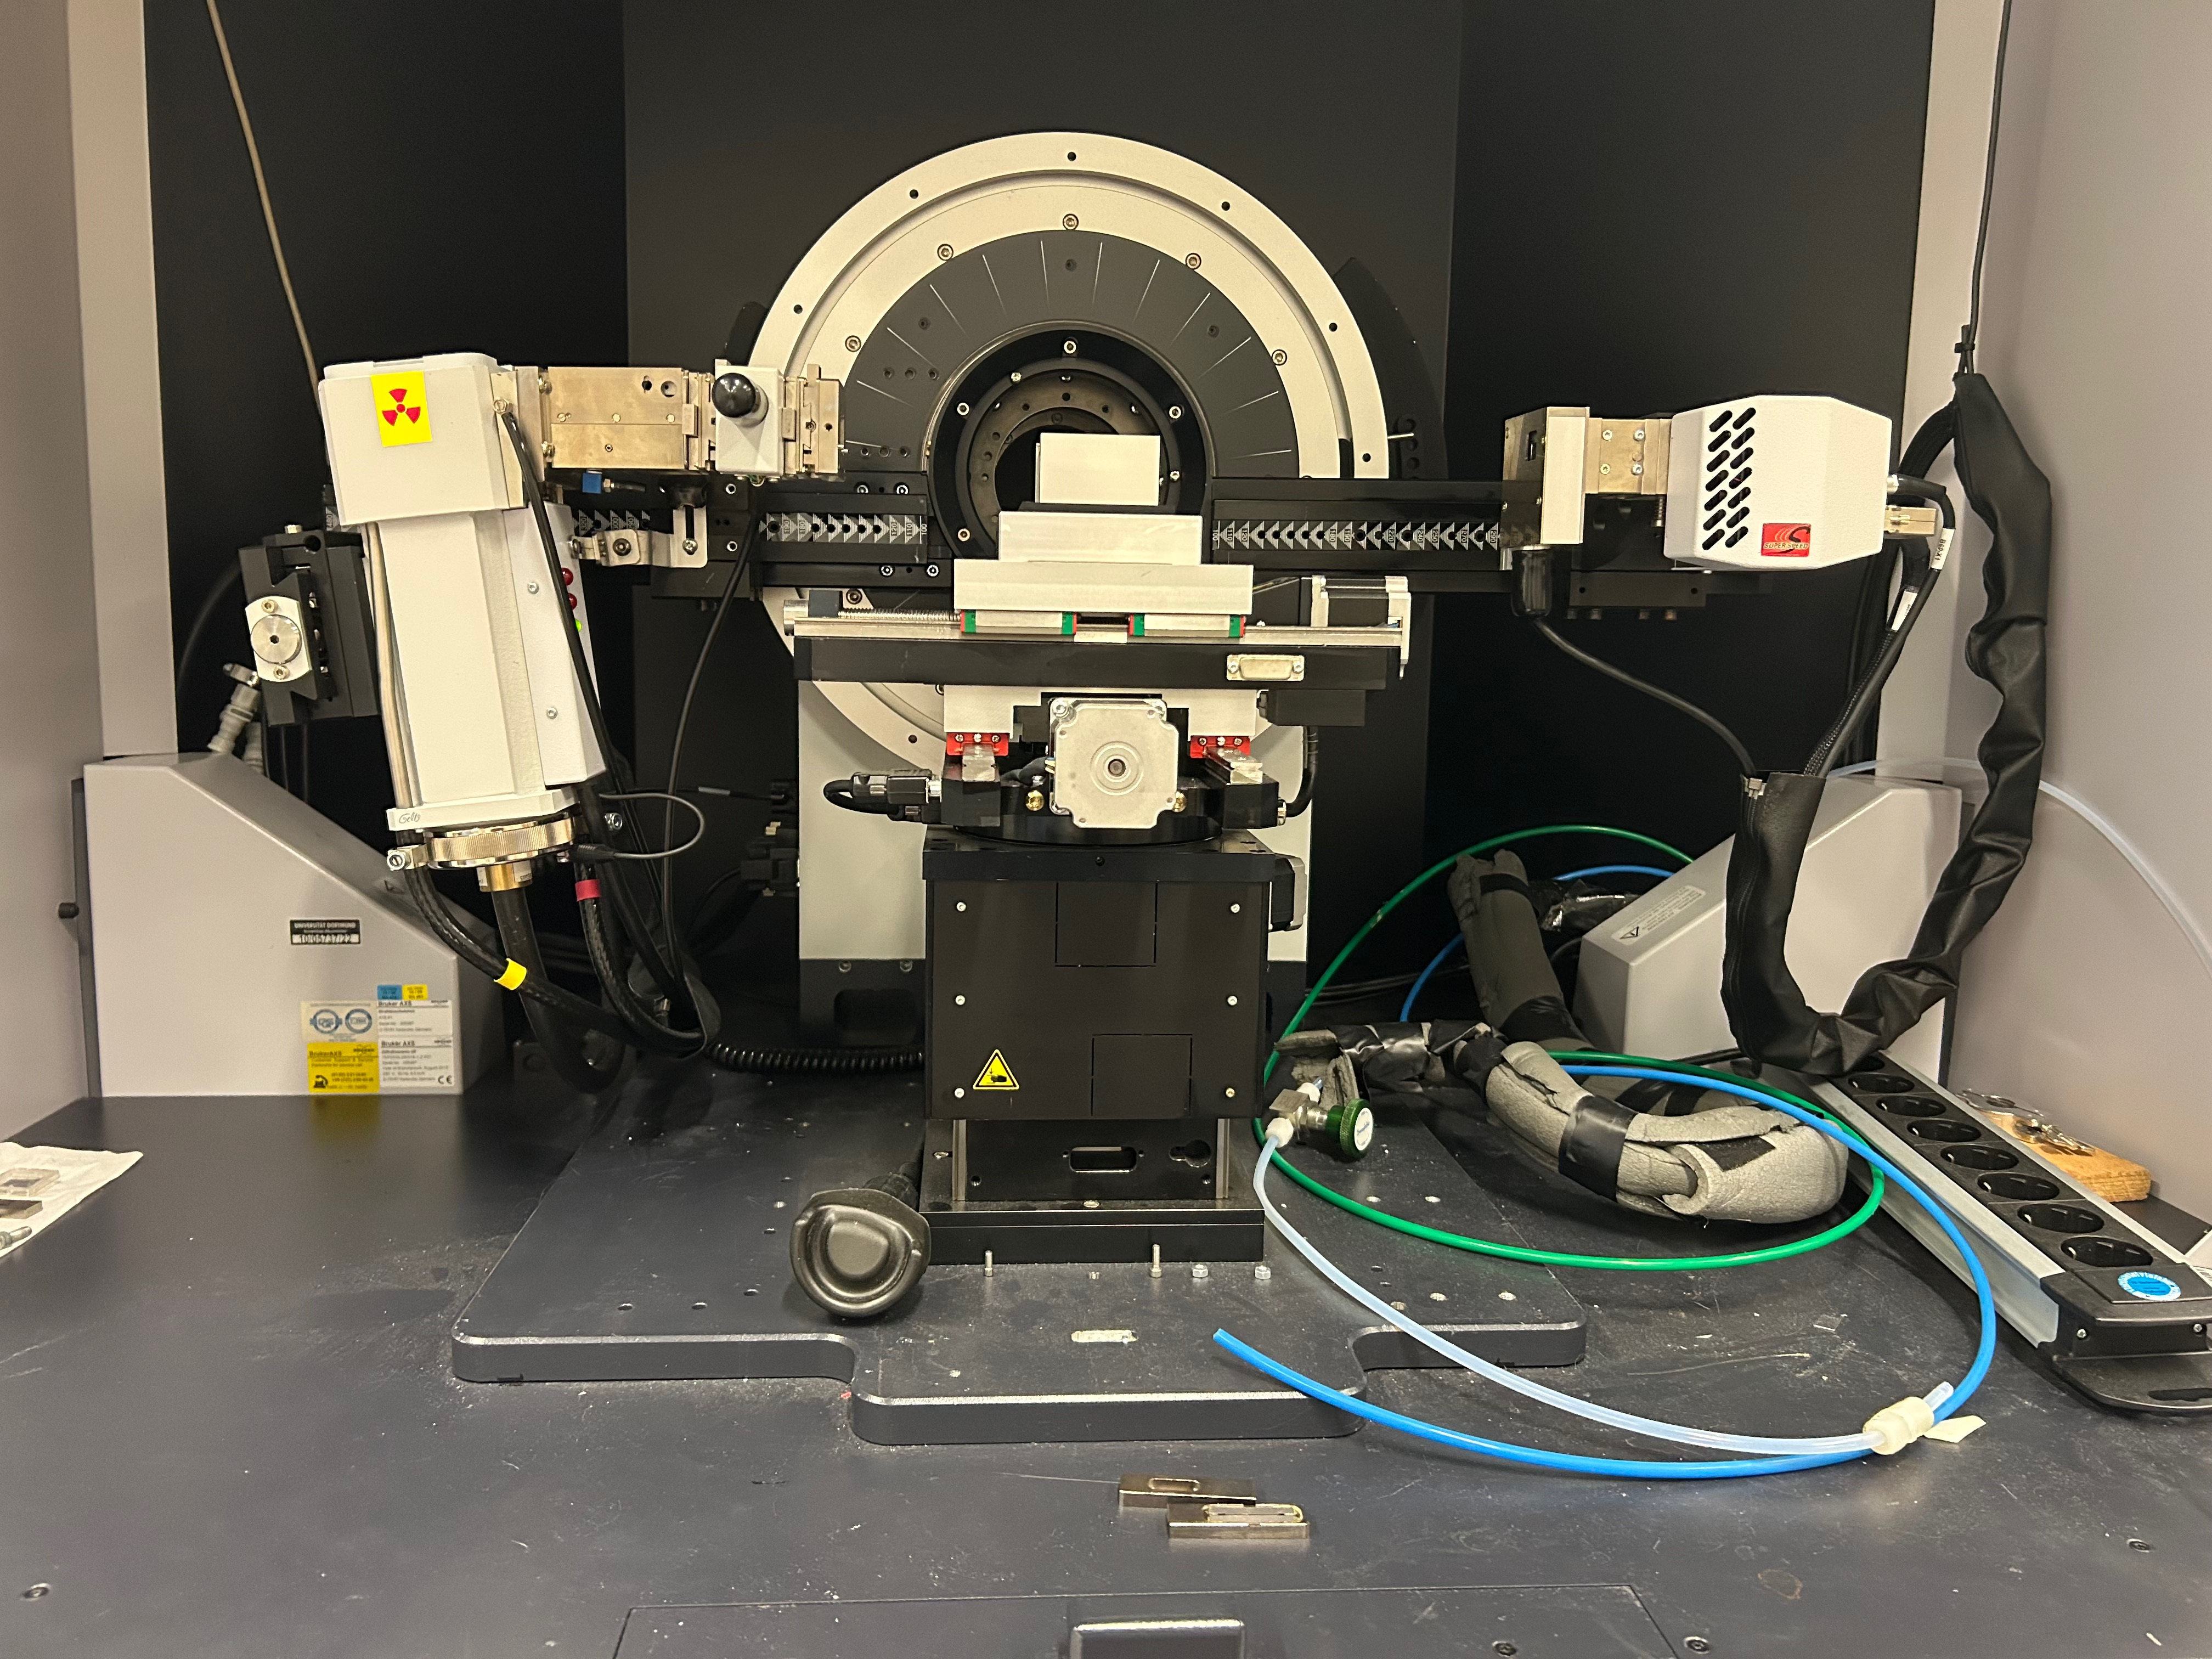
\includegraphics[width=\textwidth]{bilder/aufbau.jpeg}
    \caption{Der Versuchsaufbau zur Bestimmung der Strukturmerkmale
    eines Polystyrolfilms auf einem Siliziumwafer.}
    \label{fig:Abbildung 5}
\end{figure}


\begin{figure}[H]
    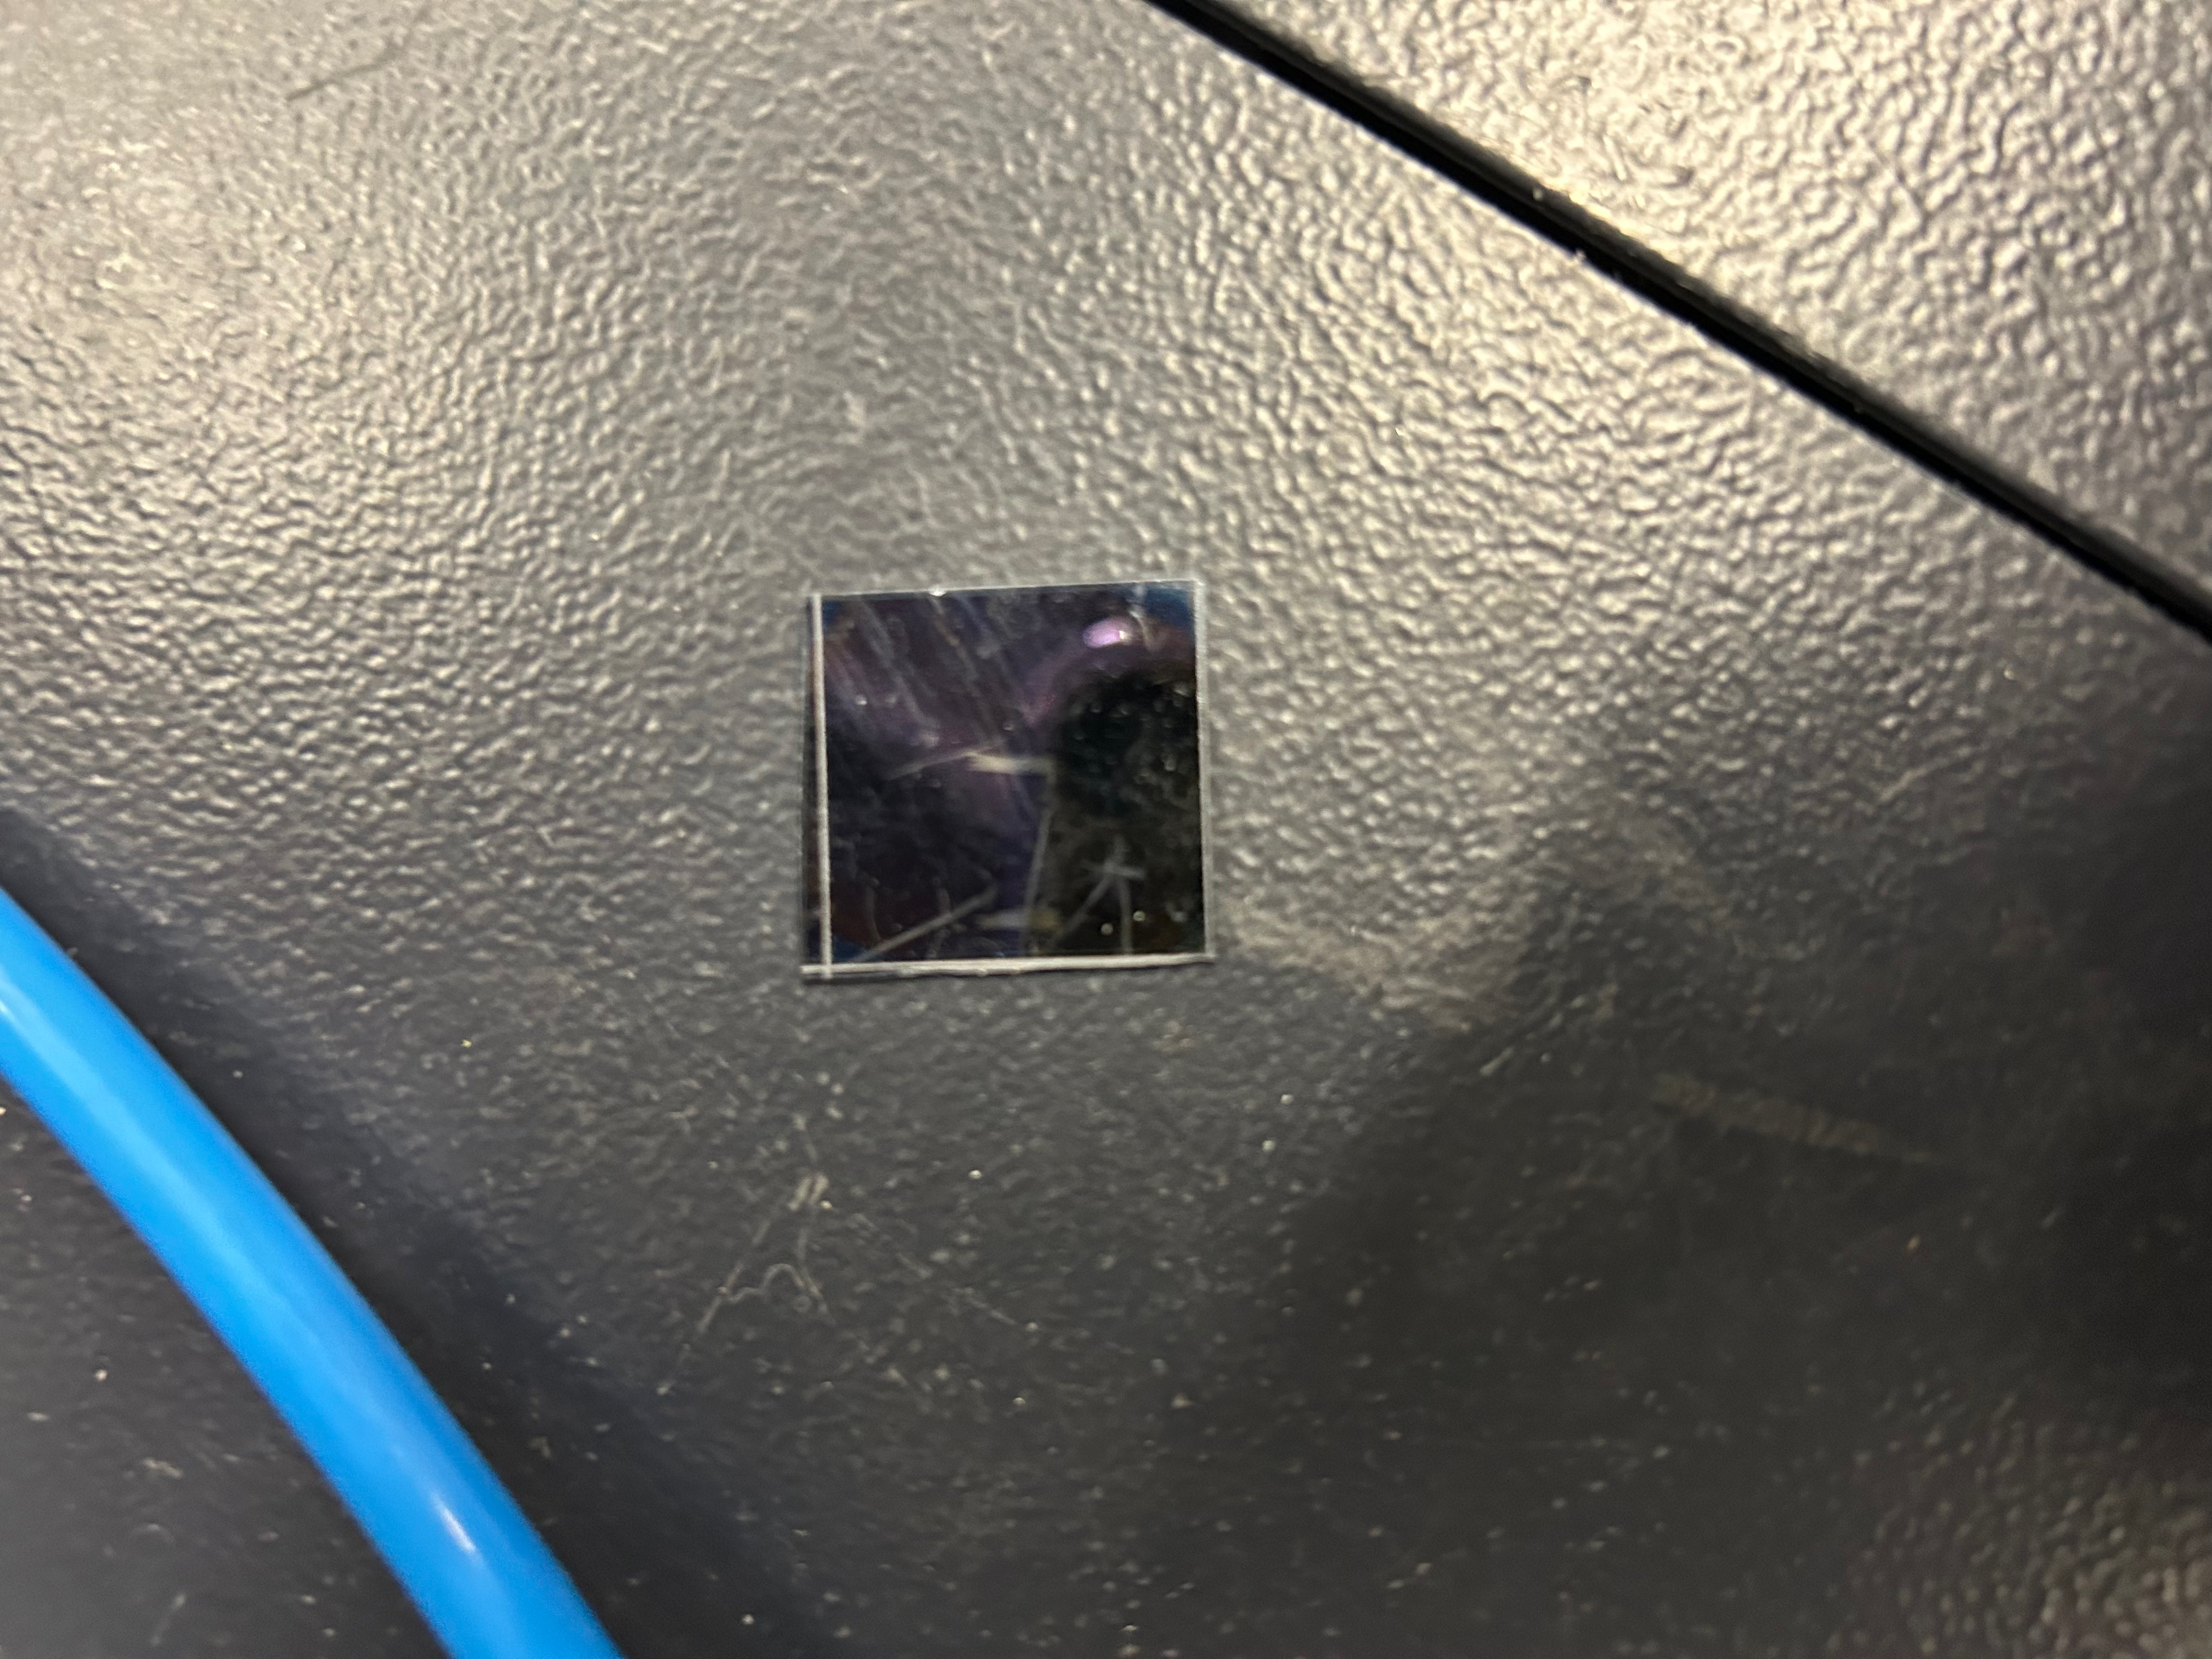
\includegraphics[width=\textwidth]{bilder/probe.jpeg}
    \caption{Der Silizumwafer beschichtet mit einem Polymerfilm.}
    \label{fig:Abbildung 6}
\end{figure}

\subsection{Justage}
Zu Beginn der Justage wird ein Detektorscan durchgefürhrt um die Null-Lage des Detektors zu bestimmen. Diese entspricht dem 
Maximum der gemessenen Verteilung. Für diese Messung wird der Probentisch vollständig aus dem Strahlengang gefahren. Die ermittelte Null-Lage wird eingestellt
und gespeichert, anschließend wird der erste Z-Scan durchgeführt. Damit wird die Position ermittelt, bei welcher die Probe die halbe Strahlintensität
abdeckt. Als nächstes wird ein x-Scan durchgeführt um sicherzustellen, dass die Probe entlang der X-Koordinate korrekt positioniert ist. Der Scan erzeugt ein Plateau 
mit verringerter Intensität. Innerhalb dieses plateaus kann je nach gewünschtem Untersuchungsbereich die genaue Position der Probe frei gewählt werden.
Ist die Probe so positioniert, dass die Intensität $\frac{1}{2}I_{max}$ beträgt, führt man einen Rockingscan durch, dabei dreht sich die Probe im Strahl.
Der scan liefert Informationen über die Verkippung der Probe im Strahl und dient dazu, die Probe in Y-Richtung in den Drehpunkt des Diffraktometers zu bringen.
Ein ideales Dreieck ist symmetrisch, wenn es asymmetrisch ist, trifft der Strahl die Probe nicht in der Mitte und die Y-Koordinate muss angepasst werden.
Ein unsymmetrisches Dreieck deutet auch darauf hin, dass die Winkeleichung der Röhre zur Probenoberfläche korrigiert werden muss. Sobald das Dreieck symmetrisch ist,
kann die Position des Maximums durch Doppelklick an die Motoren übermittelt werden. Die Röntgenröhre und der Detektor sind auf die Position eingestellt, bei der
der Rockingscan die maximale Intensität zeigt. Da diese Position meist nicht exakt bei 0 liegt, muss ein erneuter Z-Scan durchgeführt werden, um die Probe korrekt zu positionieren. 
Ein zweiter Rockingscan bei $2\theta = 0.3°$ hilft, die Justage zu verfeinern. Ein dritter Z-Scan bestimmt dann die halbe Abschattung genauer, 
indem das Intensitätsmaximum abgelesen und die entsprechende Z-Position angefahren wird. Damit ist die Probe justiert.

\subsection{Untersuchung des Polymerfilms auf einem Silizum-Wafer }
Der Messvorgang eines Polymerfilms auf einem Silizium-Wafer umfasst zwei Schritte. 
Zuerst wird ein Scan mit gleichen Einfalls- und Detektorwinkeln durchgeführt, gefolgt von einem zweiten Scan, bei dem der Detektorwinkel um 0,1° verschoben ist,
um gestreute Intensität zu bestimmen. Die Differenz zwischen den beiden Scans ergibt die wahre Reflektivität.

